%%% LaTeX Template: Two column article
%%%
%%% Source: http://www.howtotex.com/
%%% Feel free to distribute this template, but please keep to 
%%% referal to http://www.howtotex.com/ here.
%%% Date: February 2011

%%% Preamble
%%%%%%%%%%%%%%%%%%%%%%%%%%%%%%%%%%%%%%%%%%%%%%%%%%%%%%%%%%%%%%%%%%%%%%%%%%%%%%%%
\documentclass[a4paper]{article}
\usepackage[utf8]{inputenc}

\usepackage{lipsum} % Package to create dummy text

\usepackage[english]{babel} % English language/hyphenation
\usepackage[protrusion=true,expansion=true]{microtype} % Better typography
\usepackage{amsmath,amsfonts,amsthm, bm} % Math packages
\usepackage[pdftex]{graphicx} % Enable pdflatex 
\usepackage[svgnames]{xcolor} % Enabling colors by their 'svgnames' 
\usepackage[hang,small,labelfont=bf,up,textfont=it,up]{caption} % Custom captions under/above floats 
\usepackage{epstopdf} % Converts .eps to .pdf 
\usepackage{subfig} % Subfigures 
\usepackage{booktabs} % Nicer tables 
\usepackage{fix-cm} % Custom fontsizes
\usepackage{multirow} % Multiple rows
\usepackage[margin=2cm]{geometry}



\title{Coursera Capstone Project: Word prediction }
\author{David Pham}
\date{September 2014}

\usepackage{natbib}
\usepackage{graphicx}

\newcommand{\R}{\textsf{R}}

\date{September 19, 2014} % No date

\begin{document}

\maketitle

\section{Introduction}
Within the data specialization track offered by Coursera, instructors challenged
us, the students, to produce a statistical data-product  using \R able to
predict the end of sentence of sequence of words. This has extremely useful
application in text input on smartphones as the new feature of iOS 8 allowing
for alternative keyboards  demonstrates. 
In this report, a summary of the data, presenting the main challenge of the
project, and main methods will be introduced.

\section{Data}
Although other languages (among German and Russian) were available, only English
has been chosen for this study. Reasons for this choice are that there are
already several challenge and choice that need to be addressed before going in
more difficult territories.

Three types of raw texts (english news, blogs entries, users' tweets) have been
made available to download (about 500mb of data). Each observation being
separated by an end of line. 

\begin{table}
{\small
\centering
\begin{tabular}{rrrrrrl}
  \hline
 & messages & med.words & mad.words & med.chars & mad.chars & dataset \\ 
  \hline
1 & 1010242 & 31 & 19.27 & 184 & 117.13 & news \\ 
  2 & 899288 & 29 & 32.62 & 158 & 180.88 & blogs \\ 
  3 & 2360148 & 12 & 7.41 & 65 & 45.96 & twitter \\ 
   \hline
\end{tabular}
\caption{Summary statistics of the data sets, based on a sample of $10^5$
   observations for each text.}
}
\end{table}

Thanks to the huge number of observations per text, number of words per
observation after a log-transformation are well summarized by gaussian
distribution.

Quantitatively speaking, one observes that number of words on blogs entries have
a bigger variance than english news, although they have approximately the same
number of words in mean to the contrary the \textit{twitter} dataset, with a lot
less number of words. Concerning the type of text, preliminary exploratory
analysis did not reveal anything in particular, they seems to display the same
level of english complexity. 

One remarks that although these data sets are labeled English, there have a lot
of uncommon (non-ascii) characters (Japanese, Korean and Chinese as well) which
makes the analysis harder. Note that as the data are raw, spelling mistakes are
still in the text, adding noise (or information depending on which point of
view). 

\begin{figure}[h!]
\centering
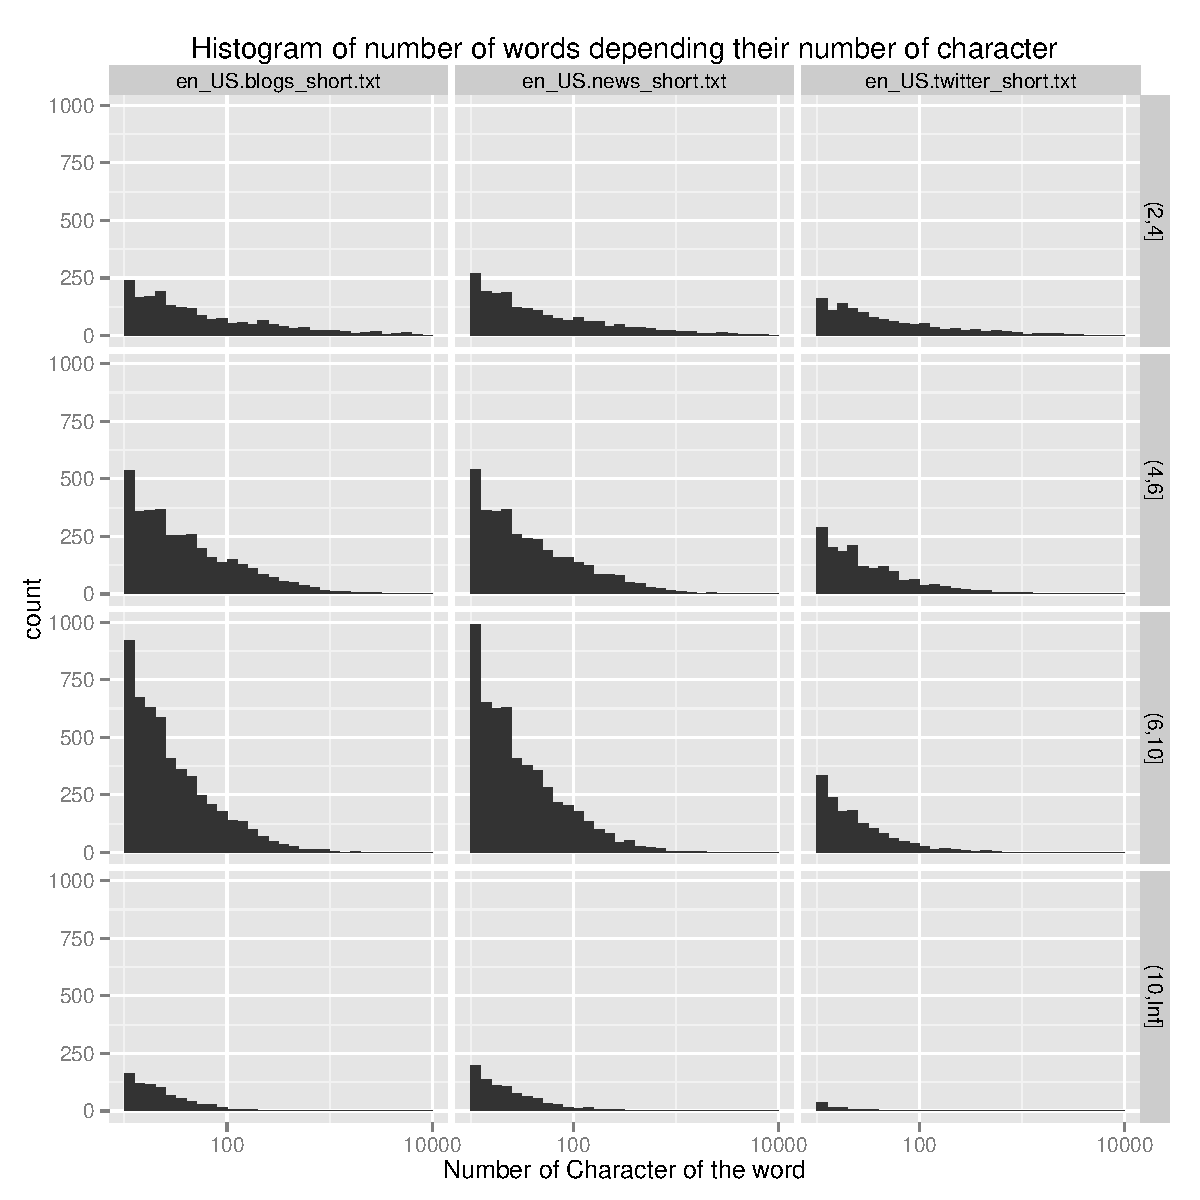
\includegraphics[width=0.45\textwidth]{plots/hist_num_char.pdf}
\caption{Count of number of words by text type and number of characters}
\label{fig:character_per_words}
\end{figure}


\section{Methodology}
\paragraph{Data cleaning}
The following procedures have performed:
\begin{itemize}
  \item Removal of bad words using the dictionary shared with the other students;
  \item Almost all punctuation has been removed: ``-'' and ``' ''  has been kept
    as they have a different meaning in English;
  \item As English is the main language of study, all letters have been
    transformed to lower cases;
  \item Numbers have been removed;
  \item White space have stripped from observations;
  \item All non-ascii character have been deleted.
\end{itemize}
\paragraph{Technological choices}
To lead the project, \R has been chosen/imposed as the default choice. Several
packages will be useful:
\begin{description}
\item[tm] An environment to clean and manage text file data
\item[tau] Library allowing to make really fast text counting for natural
  language processing technics.
\item[Matrix] Sparse matrix data structure
\item[ggplot2] Data visualization
\item[parallel] Speed improvement;
\item[data.table] Data structure mimicking the data.frame, but with thousand
  times faster performance.
\end{description}
The main problem with using \R is it does not provide a convenient dictionary
structure as python for example. One could certainly use the environment data
structure or even lists, however looking up demand a huge amount of time to
perform the analysis.
\section{Learning and Prediction Methods}
The main challenge are the following:
\begin{itemize}
\item What data structure to use in order to summarize the data?
\item How to predict words we did not yet observe?
\item How complex will the model be? What are the trade-off between biais and variance? 
\item What is the performance in real time situation of the model?
\end{itemize}
To begin with, models with tri- and bigram will be used (sequence of three and
two words). Good-Turing and
Back-off techniques will used to adjust for non observed realizations.
Good-Turing correction basically corrects the observation biais while the
Back-off algorithm provides a smart way to smooth the data to account for unseen
observation. These steps require a lot of look-up operations which are really
slow in \R, making one of the bottleneck of the learning process. 

A first result will provide a static model (the model will learn only once and
be run for a certain amount of time to see how well it performs.)

\section{Conclusion}
As the structure of the data is quite uncommon for a statistician, the challenge
offered by this project is tremendous. Even though we are at the genesis of the
project, we have a lot of hope that the products of our analysis will be
displayable online and testable by other people. Finally, let us not that R is
not the most appropriate language to create a good word prediction device.

\end{document}
